\documentclass[a4paper, 12pt]{report}
\usepackage{cmap}
\usepackage{amssymb}
\usepackage{amsmath}
\usepackage{graphicx}
\usepackage{amsthm}
\usepackage{upgreek}
\usepackage{setspace}
\usepackage{color}
\usepackage{moreverb}
\usepackage[T2A]{fontenc}
\usepackage[utf8]{inputenc}
\usepackage[normalem]{ulem}
\usepackage{mathtext} % русские буквы в формулах
\usepackage[left=2cm,right=2cm, top=2cm,bottom=2cm,bindingoffset=0cm]{geometry}
\usepackage[english,russian]{babel}
\usepackage[unicode]{hyperref}
\newenvironment{Proof} % имя окружения
{\par\noindent{$\blacklozenge$}} % команды для \begin
{\hfill$\scriptstyle\boxtimes$}
\newcommand{\Rm}{\mathbb{R}}
\newcommand{\Cm}{\mathbb{C}}
\newcommand{\Z}{\mathbb{Z}}
\newcommand{\I}{\mathbb{I}}
\newcommand{\N}{\mathbb{N}}
\newcommand{\rank}{\operatorname{rank}}
\newcommand{\Ra}{\Rightarrow}
\newcommand{\ra}{\rightarrow}
\newcommand{\FI}{\Phi}
\newcommand{\Sp}{\text{Sp}}
\renewcommand{\leq}{\leqslant}
\renewcommand{\geq}{\geqslant}
\renewcommand{\alpha}{\upalpha}
\renewcommand{\beta}{\upbeta}
\renewcommand{\gamma}{\upgamma}
\renewcommand{\delta}{\updelta}
\renewcommand{\varphi}{\upvarphi}
\renewcommand{\phi}{\upvarphi}
\renewcommand{\tau}{\uptau}
\renewcommand{\lambda}{\uplambda}
\renewcommand{\psi}{\uppsi}
\renewcommand{\mu}{\upmu}
\renewcommand{\omega}{\upomega}
\renewcommand{\d}{\partial}
\renewcommand{\xi}{\upxi}
\renewcommand{\epsilon}{\upvarepsilon}
\newcommand{\intx}{\int\limits_{x_0}^x}
\newcommand\Norm[1]{\left\| #1 \right\|}
\newcommand{\sumk}{\sum\limits_{k=0}^\infty}
\newcommand{\sumi}{\sum\limits_{i=0}^\infty}
\newtheorem*{theorem}{Теорема}
\newtheorem*{cor}{Следствие}
\newtheorem*{lem}{Лемма}
\begin{document}
	% Оформление титульного листа
	\begin{titlepage}
		\begin{center}
			\textsc{МИНИСТЕРСТВО ОБРАЗОВАНИЯ РЕСПУБЛИКИ БЕЛАРУСЬ БЕЛОРУССКИЙ ГОСУДАРСТВЕННЫЙ УНИВЕРСИТЕТ
				\\[5mm]
				ФАКУЛЬТЕТ ПРИКЛАДНОЙ МАТЕМАТИКИ И ИНФОРМАТИКИ\\[2mm]
				Кафедра информационных систем управления
			}
			
			\vfill
			
			\textbf{Отчет по лабораторной работе №3\\
				Вариант 12
				\\[26mm]
			}
		\end{center}
		
		\hfill
		\begin{minipage}{.5\textwidth}
			\begin{flushright}
				Бовта Тимофея Анатольевича\\
				студента 3 курса\\
				специальности «прикладная математика»\\[5mm]
				
				Преподаватель:\\[2mm] 
				Д. Ю. Кваша\\
			\end{flushright}
		\end{minipage}%
		\vfill
		\begin{center}
			Минск, 2024\ г.
		\end{center}
	\end{titlepage}
	\newpage
	\section*{Лабораторная работа №3}
	\subsection*{Задача 1.}
	$N$ шестеpенок пpонумеpованы от 0 до N $(N\leq 10)$. Задана матрица соединений паp шестеpенoк в виде $C[i,j]=1$, если шестеpня с номеpом $i$ находится в зацеплении с шестеpней $j$, где $1\leq i<j\leq N$ . Можно ли повеpнуть шестеpню с заданным номеpом? Если да, то найти количество шестеpен, пpишедших в движение.
	\subsubsection*{Программная реализация алгоритма.}
	\listinginput[1]{1}{task1.py}
	\subsection*{Задача 2.}
	Имеется страна с N городами. Между некоторыми парами городов построены магистрали. Длина любого прямого соединения равна единице. Движение по магистрали возможно в
	обе стороны. Систему магистралей будем называть чётно-нечётной, если каждая пара различных городов соединена маршрутом как чётной длины, так и нечётной (причём маршрут
	может проходить через один город несколько раз). Необходимо определить, является ли система магистралей чётно-нечётной. Если ответ на вопрос отрицательный, то нужно найти одно
	из подмножеств множества городов, в котором наибольшее число элементов и которое удовлетворяет следующему условию: если какие-либо два различных города из этого подмножества
	соединены маршрутом, то его длина чётна.\\\\
	\textbf{Формат входных данных}\\
	Первая строка содержит число $N$ городов $(1 \leq N \leq 300)$. Следующие $N$ строк файла
	задают магистрали: $(i + 1)$-я строка содержит номера городов, которые связаны напрямую
	7
	с городом $i$ (если таких городов нет, то строка содержит нуль; числа в строке разделены
	пробелами).\\\\
	\textbf{Формат выходных данных}\\
	Если система магистралей является чётно-нечётной, то выведите единственную строку
	YES. В противном случае в первой строке выведите NO, а во второй — мощность описанного наибольшего подмножества.
\begin{figure}
	\centering
	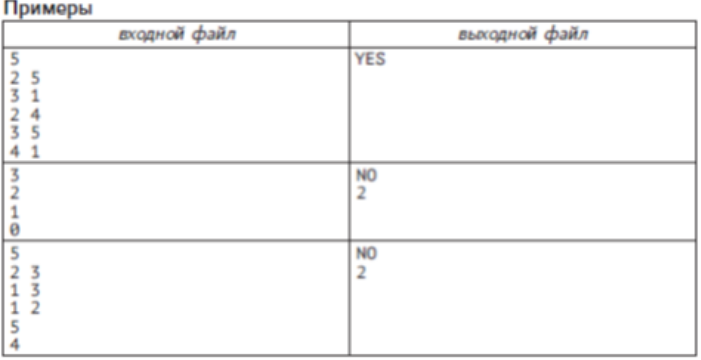
\includegraphics[scale=0.5]{screenshot001}
	\caption{}
	\label{fig:screenshot001}
\end{figure}
	
	\subsubsection*{Программная реализация алгоритма.}
	\listinginput[1]{1}{task2.py}
\end{document}